% CLASE 1
\label{CLASE1}
\section{Introducción}
\subsection{Distribución de Zona}
\begin{table}[H]
	\centering
	\caption{Zona}
	\begin{tabular}{||c||c|c||}
		\hline
		\hline
		$5$ & Tareas & $45$ \\
		$2$ & Parciales & $30$ \\
		$5$ & Parciales Sorpresa & $5$ \\
		$1$ & Final & $20$ \\
		\hline
		 & Total & $100$ \\
		\hline
		\hline
	\end{tabular}
	\label{zonas}
\end{table}


\subsection{Clases Introductorias}
\subsubsection{Surgimiento de los complejos}

Los números complejos, surgen (en los cursos), a partir de las ecuaciones cuadráticas, tales como:
	$$x^2 + 1 = 0$$
Históricamente, nacen a partir de las ecuaciones cúbicas. \\

Los complejos son un campo, claramente cumple las propiedades de un campo. Además, los complejos forman un espacio vectorial de dimensión $2$ sobre los reales (esto es claro gracias al polinomio minimal). Sabiendo la dimension del EV de los complejos, se escribe un vector cualquiera como combinación lineal de la base, i.e.
	$$z = a+bi$$
Notese que, $\Re{z} = a$ e $\Im{z} = b$, ambas son reales.

% CLASE 2
\label{CLASE2}
\subsubsection{Propiedades Algebraicas de los Complejos}
\paragraph{Conjugados}

El conjugado es el reflejo del número complejo, respecto al eje real. Es decir:
	$$z = a + bi \, \Rightarrow \, \bar{z} = a - bi$$
El signo de la parte imaginaria cambia.


\paragraph{Módulo}

Es el tamaño del vector, es decir, la hipotenusa del triangulo generado por la parte real y la parte imaginaria. Además, el módulo de $z$ es igual al módulo de su conjugado.

\dsnote{Además, se puede encontrar multiplicando el número por su conjugado, i.e. $z\bar{z} = \abs{z} ^2$}


\paragraph{Argumento}

El argumento es el ángulo que hay a partir del eje real positivo. (también es denotado por $\theta$). Esta función esta definida para $\C \setminus \{ 0 \}$. \\

También se tiene que, el argumento es el mismo independientemente de cuantas vueltas se den, es decir:
	$$\text{arg} (z) = \theta + 2k\pi$$
Con $k\in \Z$. De todos estos posibles argumentos, se tiene el \textbf{Argumento Principal}; el cual se define como: el argumento el que esté en el intervalo $(-\pi ,\pi]$, al que denotaremos como:
	$$\text{Arg} (z)$$


\subsubsection{Notación para los Complejos}

\paragraph{Notación Polar o Trigonométrica}

Tomando $\theta = \text{arg} (z)$, se tiene que:
	$$a = \abs{z} \cos{\theta}$$
	$$b = \abs{z} \sin{\theta}$$
Para simplificar la notación se define $\text{cis} \theta = \cos{\theta} + i\sin{\theta}$, con lo que
	$$z = \abs{z} \text{cis} \theta$$

\paragraph{Notación Exponencial o Euleriana}

$$z = \abs{z} e^{i\theta}$$

\dsnote{Más adelante se ahondará más en esta notación.}


\subsubsection{Propiedades}

Propiedades de los números complejos: $z,w\in \C$

\begin{enumerate}[1)]
	\item $\abs{z} = \abs{\bar{z}}$
	\item $z\bar{z} = \abs{z} ^2$
	\item $z + \bar{z} = 2 \Re{z}$
	\item $z - \bar{z} = 2\Im{z} i$
	\item $\Re{z} \leq \abs{z}$
	\item $\Im{z} \leq \abs{z}$
	\item $\bar{\bar{z}} = z$
	\item $\overline{z + w} = \bar{z} + \bar{w}$
	\item $\overline{zw} = \bar{z} \bar{w}$
	\item $\abs{z+w} \leq \abs{z} + \abs{w}$
		\begin{proof}
			Desigualdad Triangular: \\
			\begin{align*}
				\abs{z+w} ^2 &= (z+w)\overline{(z + w)} \\
				&= (z + w)(\bar{z + \bar{w}}) \\
				&= \abs{z} ^2 + \abs{w}^2 + z\bar{w} + \overline{z\bar{w}} \\ 
				&= \abs{z} ^2 + \abs{w}^2 + 2\Re{z\bar{w}} \\
				&\leq \abs{z} ^2 + \abs{w}^2 + 2\abs{z} \abs{\bar{w}} \\
				\abs{z+w} &\leq \abs{z} + \abs{w}
			\end{align*}
		\end{proof}
\end{enumerate}


% CLASE 3
\label{CLASE3}
\subsubsection{El Infinito en los Complejos}

Así como en los reales, existen relaciones de orden, en $\C$ no, no existe una comparación de orden en los números complejos. Esto es más claro analizando la propiedad de tricotomía:
\begin{description}
	\item[$i = 0$] Si la unidad imaginaria fuera cero, entonces no tendría sentido hablar de números imaginarios.
	\item[$i>0$] Si un número es positivo, la desigualdad, al multiplicarla por un positivo, se mantiene. Esto no sucede al multiplicar $i$ (considerandolo positivo) por la desigualdad $i > 0$. Por lo que $i$ no es positivo.
	\item[$i < 0$] Similarmente, con los números negativos. Si se multiplica un número negativo por una desigualdad, esta cambia de "lado". Realizando esto con $i$ (considerandolo negativo) por la desigualdad $i < 0$, se tiene una contradicción. Por lo que, $i$ no es negativo.
\end{description}

Con esto es claro que en los números complejos no hay relaciones de orden. \\

Así como en los reales se tienen dos infinitos (los infinitos no pertenecen a los reales), el negativo y el positivo. En los complejos se tienen inifinos en todas las direcciones, se tienen, infinitos infinitos.

\paragraph{Geometría Proyectiva: } A diferencia de la geometría euclideana, es el postulado de las rectas paralelas. En la geometría proyectiva, dos rectas paralelas si se intersectan. \\

El espacio proyectivo se define como:
	$$\mathbb{P} ^n _\mathbb{K} := \frac{\mathbb{K} \setminus \{ 0 \}}{\sim}$$

Con la relación de equivalencia:
	$$(x_o,\ldots ,x_n) \sim (y_o , \ldots, y_n)$$
	
Si existe $\lambda \neq 0$ tal que
	$$(x_o,\ldots ,x_n) = \lambda (y_o , \ldots, y_n)$$

\subparagraph{Ejemplo: } Tomando $\mathbb{P} ^1 _\R$, es el conjunto de rectas, en $\R ^2$, que pasan por el origen. En general, $\mathbb{P} ^n _\R$, es el conjunto de rectas, $n-$dimensionales, que pasan por el origen. Esto se cumple para más espacios vectoriales.

\dsnote{Se cumple para más espacios vectoriales? Cómo sería algebraicamente?}

Tomando la recta real paralela al eje vertical, es el conjunto que contiene un punto de todas las rectas, excepto del eje vertical. Por lo que:

	$$\mathbb{P} ^1 _\R \cong \R \cup \{ p \} \cong \R \cup \{ \infty \} \cong \text{Circunferencia}$$

Todo es isomorfo a la circunferencia puesto que la circunferencia contiene un punto de todas las rectas, incluyendo la recta "infinito". \\

Para los complejos:
	$$\mathbb{P} ^1 _\C \cong \C \cup \{ \infty \}$$
	

Siguiendo con la idea de la circunferencia, como los complejos "tienen" una dimensión más:
	$$\mathbb{P} ^1 _\C \cong \text{Esfera}$$
	
Esta esfera, es la conocida Esfera de Riemann. Esta esfera es secillo de ver su generación, si se deforma el espacio complejo todo hacia un punto en un eje vertical perpendicular a dicho espacio complejo. 

\begin{figure}[H]
	\centering
	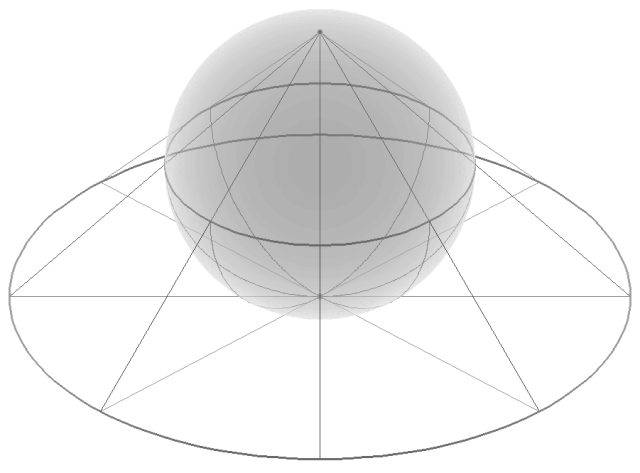
\includegraphics[scale=0.5]{Images/riemannSphere.png}
	\caption{Proyección Estereográfica}
	\label{proy_estereografica}
\end{figure}

Como esta esfera es isomorfa al espacio complejo, existe un isomorfismo entre la esfera y el plano, de modo que todo punto en la esfera tiene asociado un único punto en el espacio complejo.


% CLASE 4
\label{CLASE4}
\subsubsection{Proyección Estereográfica}

Como $\C \cup \{ \infty \} \cong \text{Esfera de Riemann}$, entonces existe un isomorfismo entre ambos espacios. Entonces, a cada punto de la esfera $x_1 ^2 + x_2 ^2 + x_3 ^2 = 1$, se le asocia $z = \flatfrac{(x_1 + ix_2)}{(1 - x_3)}$, es decir: dado $(x_1,x_2,x_3) \in \text{Esfera de Riemann}$
	$$(x_1,x_2,x_3) \mapsto \frac{x_1 + ix_2}{1 - x_3}$$
Para demostrar que dicha transformación es invertible, tomamos el módulo de la parte izquierda:
	$$\abs{z} ^2 = \frac{x_1 ^2 + x_2 ^2}{(1 - x_3)^2}$$
Como dicho punto pertenece a la esfera, entonces se tiene:
	$$ = \frac{1 - x_3 ^2}{(1 - x_3)^2} = \frac{1 + x_3}{1 - x_3}$$
Despejando $x_3$, se tiene:
	$$x_3 = \frac{\abs{z} ^2 - 1}{\abs{z} ^2 + 1}$$
Similarmente, se pueden encontrar expresiones para $x_1$ y $x_2$, con lo que se demuestra que es invertible. Geométricamente, al mapear un punto en la esfera, este punto pertenecerá al plano complejo y a la recta generada por el punto superior de la esfera y el punto de la esfera deseado a mapear.

\paragraph{Ejemplo: } Demostrar que todas las raíces de $p(z) = z^3 + 3z + 5$ tienen módulo mayor a $1$.

\begin{proof}
	Suponiendo que una raíz tiene módulo $\abs{z} \leq 1$, entonces $z^3 + 3z + 5 = 0$, despejando $5$ y enconetrando el módulo de ello se tiene: $\abs{5} = \abs{z^3 + 3z}$ por desigualdad triangular $\abs{z^3 + 3z} \leq \abs{z} ^3 + 3\abs{z}$, por la suposición inicial $\leq 1^3 + 3(1) \leq 4$, lo que es una contradicción, por lo que $\abs{z} > 1$.
\end{proof}
	


% CLASE 5
\label{CLASE5}
\subsection{Teorema de DeMoivre}

Utilizando la notación Eulereana para dos complejos $z,w$, con argumentos $\theta ,\alpha$. Con esto se tiene:
	$$z = \abs{z} e^{i\theta} \quad \quad w = \abs{w} e^{i\alpha}$$
Multiplicando ambos:
	$$zw = \abs{z} \abs{w} e^{i(\theta + \alpha)}$$
Con esta idea, se calcula:
	$$z^n = \abs{z} ^n e^{in\theta}$$
A esto se le conoce como el \textbf{Teorema de DeMoivre}, el cual es cierto, no solo para enteros, sino que para todos los complejos, i.e. $n\in \C$.

\subsection{Geometría Analítica en $\C$}

\subsubsection{Circunferencia}

Se define como el siguente conjunto:
	$$A = \{ z\in \C : \abs{z} = 1 \}$$
Sin embargo, para una circunferencia desplazada a $z_o$ con radio $r$, se tiene:
	$$\abs{z - z_o} = r$$

\subsubsection{Elipse}

La elipse, asi como en su definición clásica, para sus focos en los puntos $a$ y $b$, se tiene:

	$$\abs{z - a} + \abs{z - b} = k$$
Donde $z$ es todo punto sobre la elipse.

\subsubsection{Recta}

Para una recta entre dos complejos, se tiene que, tomando un parametro $t\in \R$, la recta que pasa por ambos complejos esta dada por:
	$$z + t(z + w)$$
Segmentando dicha recta, se tiene que, para la distancia entre ambos complejos, se limita $t$  a $0 \leq t \leq 1$. Y en base a esto se puede calcular el punto medio entre dos complejos, el cual es simplemente haciendo el valor de $t = 2$.

\subsubsection{Gravicentro}

Sabiendo la relación de las medianas y el gravicentro, entonces tomando los segmentos de recta, simplemente se realiza dicho procedimiento. Tomando cualquier lado (en este caso se tomará $ac$) se tiene que el punto medio entre dichos vértices es:
	$$\frac{a + c}{2}$$
Ahora, para el segmento entre este nuevo punto y el vértice restante es:
	$$b + t\qty(\frac{a + c}{2} - b)$$
Por la relación se tiene que $t = \flatfrac{2}{3}$, con esto y desarrollando se tiene:
	$$\boxed{G = \frac{a + b + c}{3}}$$
	
















